\subsection{Cobro de facturas}

\subsubsection{Cursograma}

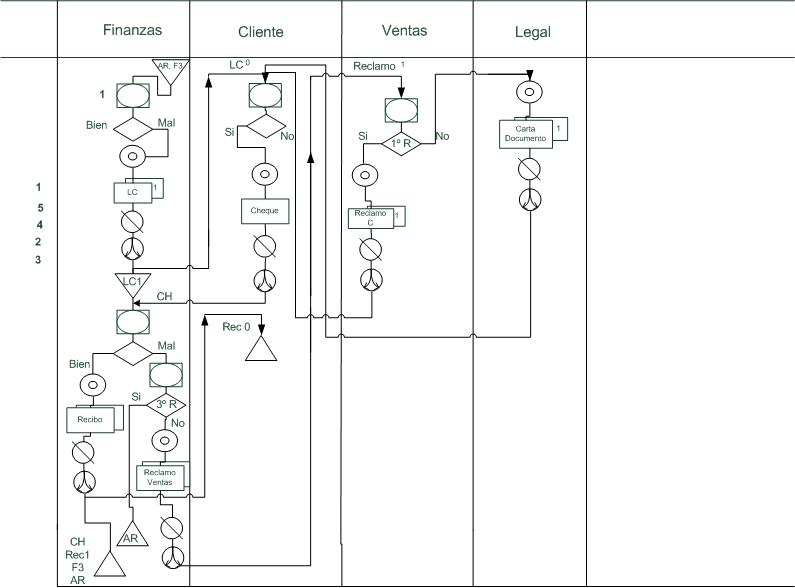
\includegraphics[scale=0.7]{Empresa/Circuitos/Cobranzas/cursograma-manual-cobranzas.jpg}

\subsubsection{Procedimiento}

\begin{enumerate}
\item El sector de Cobranzas agrupa las facturas por vencerse correspondientes seg\'un zona y clientes. Esto es avisado al sector a trav\'es del sistema de gesti\'on. Con dichas facturas agrupadas a cobrar, confecciona un listado de cobros ( LC) por duplicado.

\item El listado de cobros se envia con el cobrador al cliente. El cliente en caso de tener el cheque para pagar la factura lo entrega al cliente.

\item Si el cheque es correcto se emiten recibos por duplicado. El original es firmado por Cobranzas y se envia al cliente. El otro se guarda junto con la factura y el cheque. De esta forma el cobro finaliza y se asienta en el sistema de gesti\'on.
\end{enumerate}